\documentclass[12pt,letterpaper,noanswers]{exam}
\usepackage[usenames,dvipsnames,svgnames,table]{xcolor}
\usepackage[margin=0.9in]{geometry}
\renewcommand{\familydefault}{\sfdefault}
\usepackage{multicol}
\pagestyle{head}
\definecolor{c03}{HTML}{FFDDDD}
\header{AM 111 Class 22}{}{Skill Check}
\runningheadrule
\headrule
\usepackage{graphicx} % more modern
\usepackage{amsmath} 
\usepackage{amssymb} 
\usepackage{hyperref}
\usepackage{tcolorbox}

\begin{document}
 \pdfpageheight 11in 
  \pdfpagewidth 8.5in

\noindent Name: \rule{2.5in}{0.5pt}

\noindent Put away any notes or other materials, and work on this activity alone.

\noindent You'll receive feedback on your work and will complete a similar question on a future skill check.


\begin{questions}
\item 
Match the signal to its DFT amplitude.  Provide reasoning.

Signal:

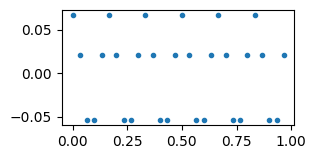
\includegraphics[width=0.3\linewidth]{img/C21skill-1.png}

Frequency options:

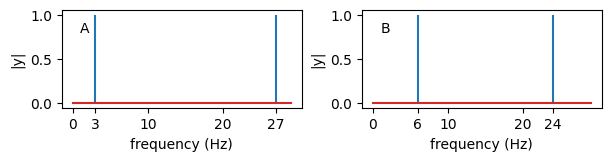
\includegraphics[width=0.7\linewidth]{img/C21skill2-1.png}

\vspace{3cm}

\item (Retake for Class 19)

Consider the initial value problem $\left\{\begin{array}{l}
y' = 3y \\
y(0) = 1
\end{array}
\right.$

Set $h = 0.2$.  Provide an expression for $y(0.2)$, as approximated using improved Euler.

\end{questions}

\end{document}